\mysection{Arrival Curves}\label{arrivalCurves}

Event stream models describe how a system is being used by the environment:
How often do events of a specific event stream arrive? Do these arrivals follow any kind of pattern? How much input data is provided to the system?
How much data is generated by the system and fed back to its environment after the processing~\cite{mar}?
To answer these questions, we have to construct an own event stream model for each stream of the system, by specifying the event bound functions.

\mysubsection{Event Bounds}

We define the differential arrival function \(R[s, t)\) as the total number of events that arrive within the time interval \([s, t): s,t \in \mathbb{R}\)~\cite{cho:08}.
While R models one concrete trace of an event stream, in the framework of RTC we usually characterize an event stream by its arrival curves~\cite{cho:08}:
\[\overline{\alpha}(\Delta t) = [\overline{\alpha}^{\, u}(\Delta t), \overline{\alpha}^{\, l}(\Delta t)] \]
These bounds are related by
\[\forall t \leq s \leq 0: \overline{\alpha}^{l}(t-s) \leq R[s, t) \leq \overline{\alpha}^{u}(t-s)\]
meaning that all possible traces of this event stream are located between the lower arrival curve \(\overline{\alpha}^{\, l}(\Delta t)\) and the upper arrival curve \(\overline{\alpha}^{\, u}(\Delta t)\).
Thus, these curves set guaranteed lower and upper bounds on the number of incoming events at this particular event stream over any time interval of length \(\Delta t\)~\cite{moy}.

In contrast to \(\overline{\alpha}(\Delta t)\), \(\alpha(\Delta t)\) describes the amount of resource capacity an event stream demands over a period of time\cite{cho:08}.
This specification is needed for most use cases and can be obtained by
\[[\alpha^{\, u}(\Delta t), \alpha^{\, l}(\Delta t)] = [\gamma^{u}(\overline{\alpha}^{\, u}), \gamma^{l}(\overline{\alpha}^{\, l})]\]
Here \(\gamma(e) = [\gamma^{u}(e), \gamma^{l}(e)]\) defines the minimum and maximum work, that is required per number of incoming event \textbf{e}~\cite{mar}.
Usually \(\gamma\) can be simplified to the basic linear function \(\gamma(e) = e \cdot WL\) with the task-specific workload of a single event being \textbf{WL}\cite{wan:06}.

%In more complex systems, the arriving events within one event stream may be of different types and therefore have different resource demands.
%These complex resource demands can then be modeled using automata~\cite{wan:06}.

\mysubsection{Handling Different Arrival Patterns}

Various event arrival patterns with deterministic timing behavior, such as sporadic, periodic and periodic with jitter, can be efficiently abstracted into curves~\cite{cha},~\cite{wan:12}.

In this paper we will focus on periodic event streams.
Within these streams there will always be exactly one event occurring within the period \textbf{p}.
In case we are observing a periodic event stream with a jitter \textbf{j}, that period p is guaranteed to be in \([p-j,p+j]\)~\cite{mar}.
It is important to notice, that those jitters do not accumulate: the 10th event will for example arrive within \([9p-j,10p+j]\), not within \([9p-9j,10p+10j]\).
Furthermore, the minimum distance \textbf{d} between the arrivals of two events needs to be specified whenever dealing with a jitter.

The arrival curves without jitter (\autoref{fig:simple_period}) and with jitter (\autoref{fig:period_with_jitter}) can now be modeled graphically or in the form of equations~\cite{wan:12}:
\[\overline{\alpha}^{l}(\Delta t)=\left\lfloor\frac{\Delta t-j}{p}\right\rfloor\]
\[\overline{\alpha}^{u}(\Delta t)=\min{\left\{\left\lceil\frac{\Delta t+j}{p}\right\rceil,\left\lceil\frac{\Delta t}{d}\right\rceil\right\}}\]
Those functions can also be approximated linearly to facilitate the upcoming calculations, yet this leads to less accurate results~\cite{wan:06}.

\begin{figure}
    \centering
    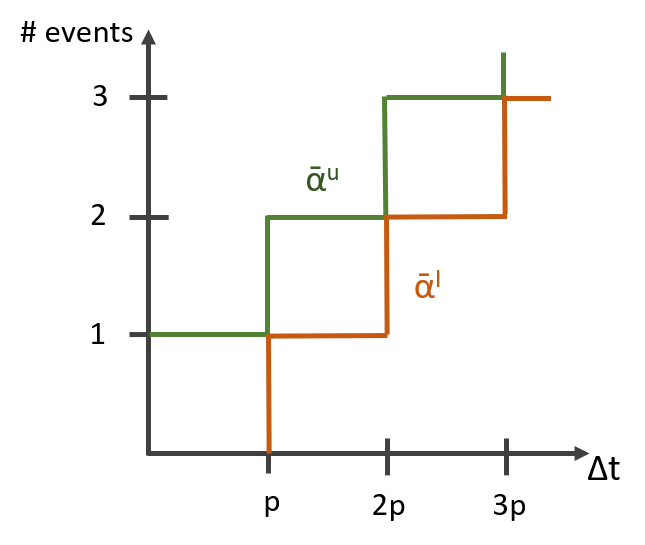
\includegraphics[width=0.7\columnwidth]{graphics/simple_period.png}
    \caption{Arrival curve with period p}\label{fig:simple_period}
\end{figure}

\begin{figure}
    \centering
    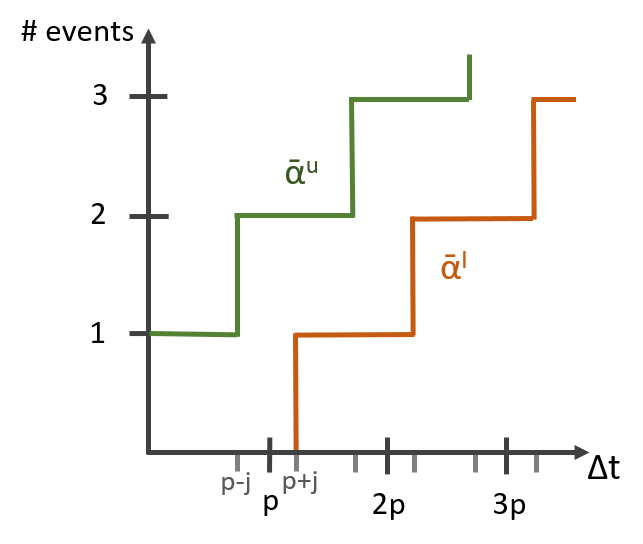
\includegraphics[width=0.7\columnwidth]{graphics/period_with_jitter.png}
    \caption{Arrival curve with period p and jitter j}\label{fig:period_with_jitter}
\end{figure}

\mysubsection{Arrival Curves of the Sample System}

As the sequence charts \autoref{fig:seq_brightness} and \autoref{fig:seq_message} define the maximum amount of incoming events per event stream and time interval,
we can easily model these streams using curves (see \autoref{fig:a-ins}).
The workload of the various tasks are also given by the sequence charts.
Therefore, we could construct the resource based arrival curves as well.

\begin{figure}
    \centering
    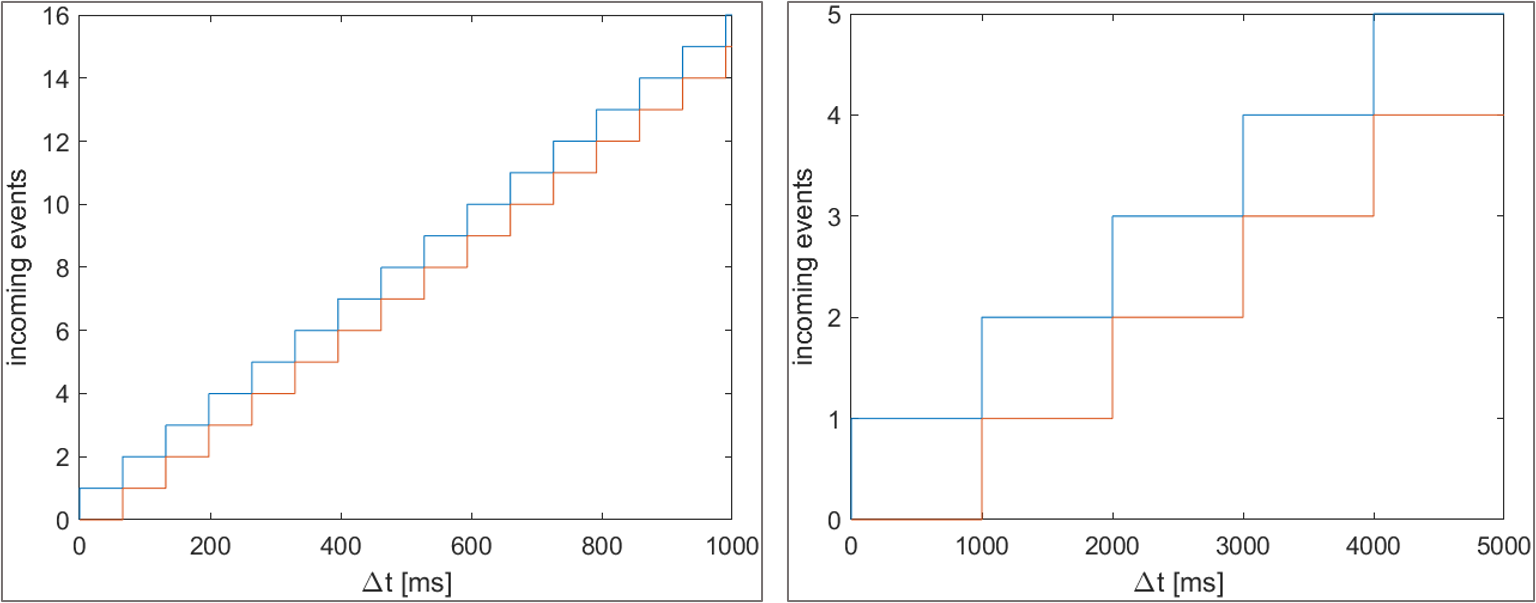
\includegraphics[width=\columnwidth]{graphics/example_a_ins.png}
    \caption{Arrival curves of brightness events (left) and message events (right)}\label{fig:a-ins}
\end{figure}